\chapter{Introduction}

\section{Overview}

\section{Sequence Evolution}

\subsection{DNA Mutation}

\subsection{Compositional Difference}

\section{Modelling Sequence Evolution}

\gls{edge}

\subsection{Phylogenetics}

\gls{floating point arithmetic}

\subsection{Introduction to Markov Models}

\gls{branch length}

\subsection{Substitution Models}

\subsection{Time-Reversibility}

\subsection{Stationarity}

\subsection{Maximum Likelihood}

\subsection{Hypothesis Tests}

\gls{strand-symmetric}

\section{Non-stationarity}

\subsection{Natural Biological Experiments}

\subsubsection{Translocation of \textit{Fxy} gene in mice}

\begin{figure}[htbp]
\centering
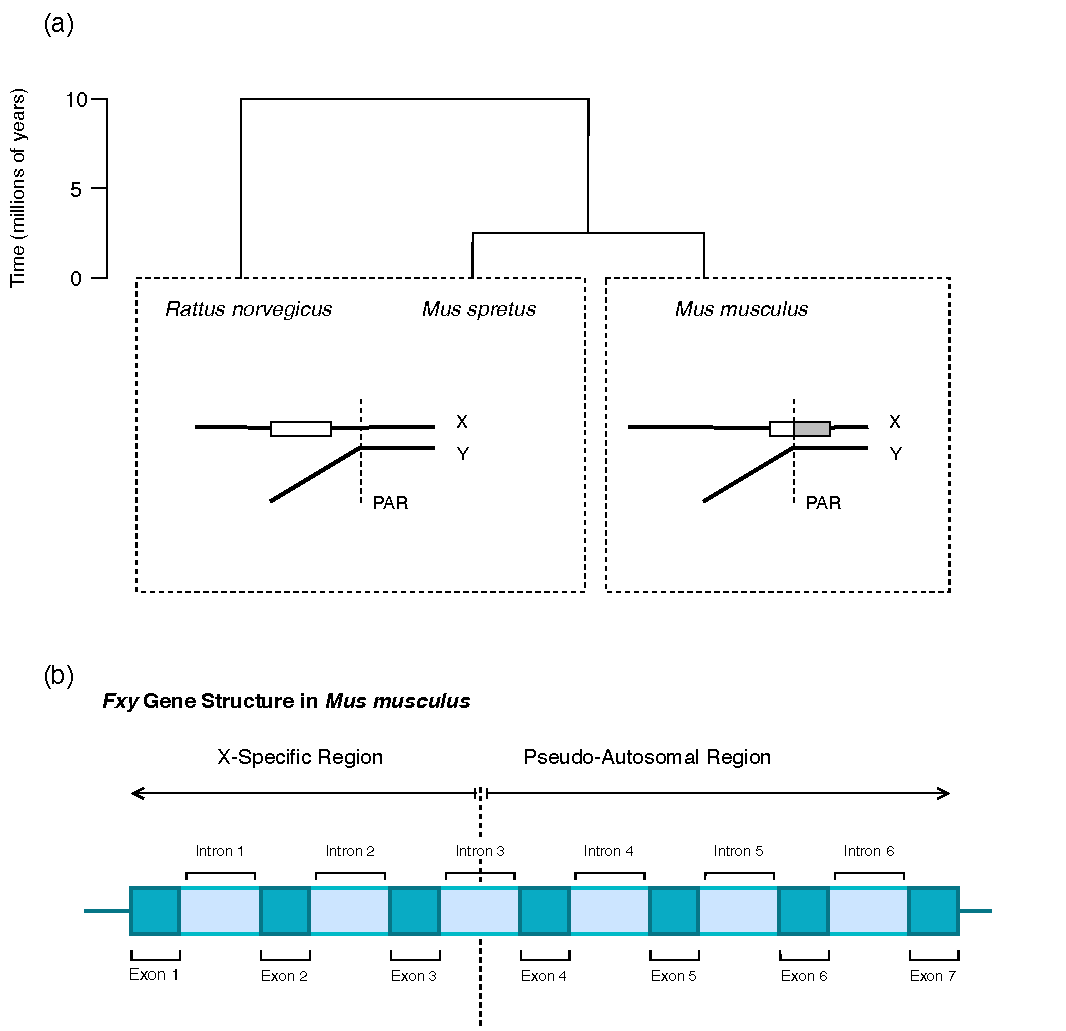
\includegraphics[width=\textwidth]{figures/diagrams/Fxy.pdf}
\caption[Evolutionary History of \textit{Fxy} in Rodents]{\textbf{Evolutionary History of \textit{Fxy} in Rodents}. \textbf{(a)} The \textit{Fxy} gene in \textit{M. musculus} was translocated from a X-specific position to a new position in which it overlaps with the PAR. The overlap in \textit{M. musculus} is shown as the shaded region of the gene, shown as a box. The divergence timescale is indicated in millions of years. In rodents and other mammals \textit{Fxy} is X-specific, suggesting translocation to the PAR in \textit{M. musculus} after divergence with \textit{M. spretus}, between 2-3 million years ago \citep[adapted from Figure 1][]{Galtier2007AdaptationEvolution}. \textbf{(b)} The structure of the \textit{Fxy} gene in \textit{M. musculus}. The $5'$ end of the gene, exons 1-3, are X-specific. The $3'$ end of the gene, exons 4-10, are positioned in the PAR. Note that for simplicity, exons beyond exon 7 are not shown in the structure. The boundary to the PAR falls in intron 3 of \textit{Fxy} \citep{Palmer1997AMice}. }
\label{fig:Fxy}
\end{figure}

\subsubsection{Loss of DNA methylation genes in \textit{Drosophila}}

\subsection{Motivate why we need to know more about these processes}

\gls{strand-asymmetric}

\section{Literature as it stands}